% CVPR 2027 submission draft. Built on the official author kit (https://github.com/cvpr-org/author-kit).
\documentclass[10pt,twocolumn,letterpaper]{article}
\usepackage[review]{cvpr}
%% This file contains a number of tweaks that are typically applied to the main document.
%% They are not enabled by default, but can be enabled by uncommenting the relevant lines.


%%
%% Official support for 2-column teaser figure
%%
\usepackage{cuted} %< for strip environment

%%
%% For auto-referencing of figures (see fig/teaser.tex and \label{} therein) 
%%
\usepackage{currfile} %< for \currfilebase macro

%%
%% caption and (global) spacing overrides
%%
\usepackage{caption} %< for "\captionof" commands (teaser)
% \setlength{\abovecaptionskip}{.5em} % space above caption
% \setlength{\belowcaptionskip}{1em} % space below caption

%%
%% Inline annotations; for predefined colors, refer to "dvipsnames" in the xcolor package:
%% https://tinyurl.com/overleaf-colors
%%
\newcommand{\red}[1]{{\color{red}#1}}
\newcommand{\todo}[1]{{\color{red}#1}}
\newcommand{\TODO}[1]{\textbf{\color{red}[TODO: #1]}}
%%
%% Disable for camera ready / submission by uncommenting these lines:
%%
% \renewcommand{\TODO}[1]{}
% \renewcommand{\todo}[1]{#1}

%%
%% Work harder in optimizing text layout. Typically shrinks text by 1/6 of page, enable
%% it at the very end of the writing process, when you are just above the page limit.
%%
% \usepackage{microtype}

%%
%% Fine-tune paragraph spacing.
%%
% \renewcommand{\paragraph}[1]{\vspace{.5em}\noindent\textbf{#1.}}

%%
%% Globally adjusts space between figure and caption.
%%
% \setlength{\abovecaptionskip}{.5em}

%%
%% Allows "the use of \paper to refer to the project name"
%% with automatic management of space at the end of the word.
%%
% \usepackage{xspace}
% \newcommand{\paper}{ProjectName\xspace}

%%
%% Commonly used math definitions.
%%
% \DeclareMathOperator*{\argmin}{arg\,min}
% \DeclareMathOperator*{\argmax}{arg\,max}

%%
%% Tighten underline.
%%
% \usepackage{soul}
% \setuldepth{foobar}

%%
%% Reconfigure paragraph (tweaks spacing)
%%

\usepackage{booktabs}
\usepackage{multirow}
\usepackage{amsmath}
\usepackage{xspace}
\definecolor{cvprblue}{rgb}{0.21,0.49,0.74}
\usepackage[pagebackref,breaklinks,colorlinks,allcolors=cvprblue]{hyperref}

\def\paperID{37948}
\def\confName{CVPR}
\def\confYear{2027}

\newcommand{\cov}[1]{cov@#1\xspace}
\newcommand{\osw}{OSWorld-G\xspace}
\newcommand{\sspro}{ScreenSpot-Pro\xspace}
\newcommand{\ssv}{ScreenSpot-v2\xspace}

\title{Beyond the Accessibility Tree: Fast, Instruction-Aware Option Lists\\from Pixels for Computer-Use Agents}
\author{Anonymous CVPR submission\\Paper ID \paperID}

\begin{document}
\maketitle
\begin{abstract}
Computer-use agents act by choosing among the elements on a screen. The accessibility (AX) trees they usually
rely on omit icons, canvas widgets and custom controls, and pixel parsers that caption every detected element are
slow and hand the agent hundreds of options. We study how to build, from pixels alone, the list of on-screen options
that a \emph{separate} decision model chooses from. Our system proposes options and never clicks, so we ask whether
the needed element is on a short list and how quickly the list is built, not whether one predicted point is
correct. Candidates come from OCR merged with a tiled detector trained on accessibility labels and a public GUI
detector; together they contain the target element for 83.8\%, 96.0\% and 98.5\% of tasks on \osw, \sspro and
\ssv. Labelling candidates costs more than detecting them, so we rank before labelling: a SigLIP model fine-tuned
on context crops with a per-screen listwise loss scores every candidate against the instruction. The top 50
candidates contain the target in 75.1\%, 81.8\% and 98.5\% of tasks (39.5\%, 31.0\% and 93.9\% when ordered by
detector confidence) and need up to 8$\times$ fewer icon captions. Ranked lists complement single-point GUI
grounders: adding a grounder's click to our scores gives lists that contain the target more often than either
alone (\sspro: 89.0\% in the top 50). An off-the-shelf VLM selector given our top 10 instead of the full candidate
list picks the right element 1.5$\times$ more often on \osw and 3.7$\times$ more often on \sspro, from prompts
4--8$\times$ shorter.
\end{abstract}

\section{Introduction}
\label{sec:intro}

At every step, an agent that operates a computer must turn an instruction (``generate the bitstream'', ``attach
the debugger'') into an action on one element of the screen. Two designs dominate. \emph{Grounding models} read the
screenshot and output a click point directly~\cite{gou2025uground,wu2024osatlas,wu2025guiactor,xie2025jedi}.
\emph{List-based agents} receive a list of candidate elements, each with a label and a location, and choose
one~\cite{deng2023mind2web,lu2024omniparser}. The list usually comes from the accessibility (AX) tree that the
operating system or browser exposes.

List-based agents have practical advantages. The chooser can be a small text model, the list can be inspected and
logged, and a chooser that is unsure can ask or try the next option. All of this depends on the list being good,
and AX trees are often incomplete: icon-only buttons, canvas content, custom-drawn toolbars and many
cross-platform frameworks expose little or nothing. Pixel parsers such as OmniParser~\cite{lu2024omniparser} fill
the gap by detecting elements and captioning each icon. On a dense professional application they return hundreds
of candidates, and captioning all of them takes longer than the decision itself.

This paper studies the component in between: \emph{building, from pixels alone, the option list that a separate
model chooses from}. Because our system never clicks, its job is to put the element the instruction refers to on a
short list, quickly. We therefore measure \emph{coverage at $K$}, the fraction of tasks whose target is among the
first $K$ options, together with latency, instead of the top-1 accuracy of a click.

\paragraph{Contributions.}
\begin{itemize}
\item We formulate instruction-aware option-list construction as a ranking problem with an explicit trade-off
between coverage, list length and latency, and evaluate it on three public grounding benchmarks with
leakage-filtered splits (\cref{sec:setup}).
\item A pixel-only candidate generator that merges OCR, a detector fine-tuned on free accessibility labels and a
public GUI detector. It lists the target for 83.8\% / 96.0\% / 98.5\% of tasks on \osw / \sspro / \ssv
(\cref{sec:candidates}).
\item An instruction-aware ranker: SigLIP~\cite{zhai2023siglip} fine-tuned on \emph{context crops} (a window
around each candidate with the candidate outlined) with a \emph{per-screen listwise} loss that uses the other
candidates on the same screen as negatives. Ranking before labelling raises \cov{50} from 31.0\% to 81.8\% on
\sspro and needs up to 8$\times$ fewer icon captions (\cref{sec:ranker}).
\item A comparison with state-of-the-art single-point grounders under the same protocol. Their clicks and our
rankings complement each other: fused, they give the highest coverage at every $K$ on all three benchmarks
(\cref{sec:grounders}).
\item A downstream test with the selector held fixed: an off-the-shelf VLM picks the right element far more often
from our top 10 than from the full unranked list (\sspro: 34.6\% vs.\ 9.4\%), with prompts up to 8$\times$
shorter (\cref{sec:selector}).
\end{itemize}

\section{Related work}
\label{sec:related}

\paragraph{Screen parsing.}
Pixel-based parsers recover element boxes from screenshots. Examples are tappability and UI-element detectors on
mobile~\cite{swearngin2019tappability,zhang2021screenrecognition}, web element detection trained on rendered
pages~\cite{wu2023webui}, and OmniParser~\cite{lu2024omniparser}, which combines OCR, a YOLO icon detector and a
Florence-2 captioner and hands the result to a large model. Screen2AX~\cite{muryn2025screen2ax} predicts a macOS
accessibility hierarchy from pixels. These systems produce a list but do not rank it for an instruction. We use
OmniParser's detector as one of our candidate sources and focus on what comes after detection.

\paragraph{GUI grounding.}
Grounding models map an instruction and a screenshot to a click point:
SeeClick~\cite{cheng2024seeclick}, UGround~\cite{gou2025uground}, OS-Atlas~\cite{wu2024osatlas},
ShowUI~\cite{lin2025showui}, Aria-UI~\cite{yang2024ariaui}, JEDI~\cite{xie2025jedi}, GUI-Actor~\cite{wu2025guiactor},
GTA1~\cite{yang2025gta1}, GUI-AIMA~\cite{zhou2025guiaima} and UI-Venus~\cite{gu2025uivenus}. GroundCUA and the
GroundNext models~\cite{feizi2026groundcua} scale grounding data with human demonstrations on desktop software.
Their output is a single point, so when the point is wrong the agent has nothing to fall back on; we show that
their point and our ranking combine well. High-resolution benchmarks such as \sspro~\cite{li2025screenspotpro}
motivated zoom-in and search strategies~\cite{li2025screenspotpro,wu2025zoomclick}. RankGround~\cite{fan2026rankground}
uses a lightweight reranker to choose which high-resolution crops a grounding model sees. There the reranker serves
the grounder, whereas our ranked list of elements is itself the output.

\paragraph{Candidate ranking for agents.}
MindAct~\cite{deng2023mind2web} ranks HTML elements with a cross-encoder before a language model chooses among
the top 50, and Prune4Web~\cite{prune4web} prunes DOM candidates with generated scoring programs. Both operate on
HTML text. The closest visual analogues are learning-to-rank for object proposals~\cite{tan2019proposalrank} and
region--text matching with CLIP-style models~\cite{zhong2022regionclip,sun2024alphaclip}. Visual prompts such as a
red circle~\cite{shtedritski2023redcircle} or a blurred surround~\cite{yang2023fgvp} tell a CLIP model which region
is meant. Our ranker applies these ideas to screen elements, with a listwise loss over all candidates of a screen.

\section{Method}
\label{sec:method}

Given a screenshot $I$ and an instruction $q$, we produce an ordered list of options
$(c_1,\dots,c_K)$, each a box with a role (text or icon) and, for the options kept, a label. A separate
\emph{selector} model receives the list and picks one option. We do not train or modify the selector.
The pipeline has three stages: candidate generation (\cref{sec:candidates}), instruction-aware ranking
(\cref{sec:ranker}) and labelling of the kept icons.

\subsection{Candidates from pixels}
\label{sec:candidates}

\paragraph{Sources.}
\emph{Text:} OCR lines (Apple Vision, accurate mode) give boxes and their strings for free.
\emph{Elements:} a detector we fine-tune on accessibility labels (below), run on the full screenshot plus
overlapping tiles of about $1280$ px when the screen is large, so that 16 px icons on a 4K screen keep their
detail. Tile detections that touch a tile edge are dropped, and the rest are merged by NMS.
\emph{Icons:} OmniParser v2's icon detector~\cite{lu2024omniparser}, run the same way, with its confidences
halved so that our detector's boxes take precedence where both fire.

\paragraph{A detector trained on free accessibility labels.}
When an application exposes its AX tree, the tree is a free but incomplete source of labels. We collected
19{,}898 deduplicated macOS screenshots of 115 applications and websites with their AX trees and split them
\emph{by application} (80 / 12 / 23 apps for train / val / test). The labels are the visible actionable AX
elements. To fill in controls that AX omits, we add boxes from a public GUI detector (GPA-GUI-Detector) with
confidence $\ge 0.5$ that overlap no AX box (IoU $<0.3$). We leave out screens with almost no AX elements, which
would teach the detector to ignore real controls. We fine-tune GPA-GUI-Detector (YOLO11m) on these labels at
$1280$ px for 15 epochs. On the 3{,}275 screens of the 23 held-out applications (\cref{tab:detector}), the
fine-tuned detector boxes more of the AX elements than the public detectors (72.6\% at IoU${\ge}0.5$ vs.\ at most
61.6\%) and is the fastest. Training on AX boxes alone gives the best box quality. Adding the GPA boxes raises the
share of AX elements whose centre falls inside some detection, which is what a click needs, from 90.0\% to 97.3\%,
at 65 instead of 49 boxes per screen.

\begin{table}[t]
\centering
\small
\setlength{\tabcolsep}{3.5pt}
\begin{tabular}{l rrrrr}
\toprule
Detector (1280 px) & mAP50 & R@.5 & centre & boxes & ms \\
\midrule
GPA-GUI-Detector & 37.1 & 56.2 & 95.7 & 58 & 57 \\
OmniParser v2 & 52.1 & 61.6 & 78.9 & 37 & 42 \\
Screen2AX$^\ast$ & 17.8 & 40.9 & 71.6 & 59 & 34 \\
Ours, AX labels only & \textbf{66.7} & 71.1 & 90.0 & 49 & 21 \\
Ours, AX + GPA labels & 62.1 & \textbf{72.6} & \textbf{97.3} & 65 & 21 \\
\bottomrule
\end{tabular}
\caption{\textbf{Detectors on held-out applications} (3{,}275 screens, 142k AX elements). R@.5: AX boxes matched at
IoU${\ge}0.5$; centre: AX boxes whose centre lies inside a detection; boxes: median per screen; ms: per image on an
A10G, untiled. $^\ast$At 640 px, its better setting.}
\label{tab:detector}
\end{table}

\paragraph{Merging.}
Sources are merged into one list. OCR lines enter first. A detection whose IoU with an existing item exceeds $0.3$,
or that encloses the centres of items no more than $1.5\times$ its area, only adds its source tag and confidence to
them; otherwise it becomes a new \emph{icon} item. Text items carry their OCR string; icons have no label yet.

\subsection{Instruction-aware ranking}
\label{sec:ranker}

A screen of a professional application yields 300--600 candidates (\cref{tab:main}). Captioning every icon is the
most expensive step of pixel parsing, and a long list also makes the selector's choice harder. We therefore rank
all candidates against the instruction first and keep only the top $K$.

\paragraph{Scoring.}
Each candidate $c$ is shown to an image encoder $f_I$ as a \emph{context crop}: a square window centred on the box,
three times its longer side (at least 96 px), clipped to the screen and resized to the encoder's input size, with
the candidate outlined in red (line width about $1/112$ of the window). The outline tells the model which element
is meant~\cite{shtedritski2023redcircle}, and the window shows its neighbours, \eg the label next to an icon or the
toolbar it sits in. The instruction is encoded by the text encoder $f_T$ and
\begin{equation}
  s(q,c) = \tau\,\langle f_T(q), f_I(\mathrm{crop}(I,c)) \rangle ,
\end{equation}
with unit-normalised embeddings and SigLIP's learned temperature $\tau$. Image embeddings are computed once per
screen and shared by every instruction on it; each new instruction costs one text embedding and a matrix product.

\paragraph{Per-screen listwise training.}
A list is good when the target ranks high among the \emph{other candidates of the same screen}, so we train
for that rank directly. For an instruction $q$ on a screen with candidates $C$ and matched targets $T\subseteq C$,
\begin{equation}
  \mathcal{L}(q) = -\log \sum_{t\in T} \frac{\exp s(q,t)}{\sum_{c\in C} \exp s(q,c)} ,
\end{equation}
which counts any matched target as correct (a target box can match several overlapping candidates). All other
boxes on the screen, including near-identical neighbouring icons, act as hard negatives. We compare against
SigLIP's pointwise sigmoid loss over the same pairs in \cref{sec:ablations}.

\paragraph{Training data.}
Instructions and target boxes come from public grounding sets that are disjoint from our evaluation benchmarks:
OS-Atlas desktop (macOS and Linux)~\cite{wu2024osatlas}, MMBench-GUI~\cite{wang2025mmbenchgui},
OmniACT~\cite{kapoor2024omniact} and WebLINX~\cite{lu2024weblinx}. We run our candidate generator on their
screenshots and mark as targets the candidates whose centre falls in the answer box or that overlap it with
IoU $>0.3$ (and are at most $4\times$ its area). This gives 4{,}816 training screens with 63{,}141 instructions;
253 further screens are held out to select the checkpoint by recall@10. Per step we keep every target and sample
up to 96 candidates and 16 instructions per screen.
We fine-tune SigLIP-Base/16 at $384$ px~\cite{zhai2023siglip} with AdamW (lr $10^{-5}$, weight decay $0.05$,
one-cycle schedule, bf16) for three epochs; held-out recall@10 rises from $0.749$ (zero-shot) to $0.958$.

\paragraph{Labelling.}
Text options are labelled with their OCR string. Only icons that survive the cut are captioned, with OmniParser's
Florence-2 captioner on the icon crop, so the captioning cost grows with $K$ and not with the number of elements
on the screen. Batched on an A10G, captioning costs about 2~ms per icon.

\section{Experiments}
\label{sec:experiments}

\subsection{Setup}
\label{sec:setup}

\paragraph{Benchmarks.}
We evaluate on \osw~\cite{xie2025jedi} (Ubuntu desktop), \sspro~\cite{li2025screenspotpro} (high-resolution
professional applications on Windows, macOS and Linux) and \ssv~\cite{cheng2024seeclick} (mobile, desktop and
web), using a fixed random sample of 500 instructions per benchmark (\osw has 510 in total), identical for all
methods. No AX information is used.

\paragraph{Leakage filtering.}
OS-Atlas, MMBench-GUI and \ssv partly share their sources. We compute a 256-bit difference hash of every
evaluation and training screenshot and drop evaluation screens within 6 bits of any screenshot the ranker was
trained on: 3 of 248 \osw screens, none of the 500 \sspro screens and 130 of 384 \ssv screens. All numbers are
reported on the remaining screens (481 / 500 / 326 instructions). Filtering changes \cov{50} by at most 0.3 points.

\paragraph{Metrics.}
\emph{Coverage at $K$} (\cov{K}) is the fraction of instructions whose target is among the first $K$ options; an
option matches the target if its centre lies in the answer box or it overlaps the box with IoU $>0.3$ while being
at most $4\times$ its area (for point answers: it contains the point). Unlisted targets count as misses at every
$K$. \emph{Listed} is coverage of the unranked, uncapped list (the ceiling of any ranking). We also report the
number of icons among the first $K$, which is the number of captions the labelling stage must compute, and
latency on one NVIDIA A10G.

\subsection{Coverage and ranking}

\begin{table*}[t]
\centering
\small
\setlength{\tabcolsep}{4pt}
\begin{tabular}{l ccc ccc ccc}
\toprule
& \multicolumn{3}{c}{\osw} & \multicolumn{3}{c}{\sspro} & \multicolumn{3}{c}{\ssv} \\
\cmidrule(lr){2-4}\cmidrule(lr){5-7}\cmidrule(lr){8-10}
Ordering & \cov{10} & \cov{50} & caps@50 & \cov{10} & \cov{50} & caps@50 & \cov{10} & \cov{50} & caps@50 \\
\midrule
Detector order (unranked) & 6.0 & 38.9 & 10 & 2.4 & 21.0 & 16 & 35.0 & 92.6 & 14 \\
Random & 9.4 & 37.2 & 33 & 3.6 & 17.6 & 42 & 35.3 & 90.2 & 20 \\
Detector confidence & 15.6 & 39.5 & 32 & 7.2 & 31.0 & 40 & 51.8 & 93.9 & 17 \\
OCR text match & 29.1 & 55.9 & 10 & 27.6 & 56.6 & 19 & 69.6 & 95.4 & 15 \\
SigLIP zero-shot, tight crops & 37.6 & 57.4 & 26 & 43.2 & 59.8 & 38 & 84.4 & 96.3 & 19 \\
SigLIP zero-shot, context crops & 43.0 & 63.4 & 30 & 43.6 & 62.0 & 39 & 80.1 & 96.9 & 19 \\
\textbf{Ours} (fine-tuned, context, listwise) & \textbf{58.8} & \textbf{75.1} & 35 & \textbf{64.8} & \textbf{81.8} & 43 & \textbf{95.1} & \textbf{98.5} & 20 \\
\midrule
Listed (uncapped, any order) & \multicolumn{3}{c}{83.8 \quad (190 options)} & \multicolumn{3}{c}{96.0 \quad (442)} & \multicolumn{3}{c}{98.5 \quad (47)} \\
\bottomrule
\end{tabular}
\caption{\textbf{Coverage of the target at list length $K$} on leakage-filtered benchmarks, all orderings over the
same candidate lists. caps@50: median number of icons in the first 50 options, \ie captions needed.}
\label{tab:main}
\end{table*}

The candidate lists contain the target for 83.8\%, 96.0\% and 98.5\% of instructions (\cref{tab:main}). Without
the instruction, their order is close to random: the first 50 options by detector confidence contain the target
for only 39.5\% / 31.0\% of \osw / \sspro instructions. Lexical matching between the instruction and OCR text helps
for text targets but cannot see icons, and an off-the-shelf SigLIP scoring the candidates zero-shot reaches only
62--63\% \cov{50} on \osw and \sspro. Our ranker keeps the target in the first 10 options for 64.8\% of \sspro
instructions and in the first 50 for 81.8\%, which is 85\% of the listed targets. Its first 50 options contain a
median of 43 icons instead of 347. \Cref{fig:covk} shows coverage at every $K$.

\begin{figure*}[t]
\centering
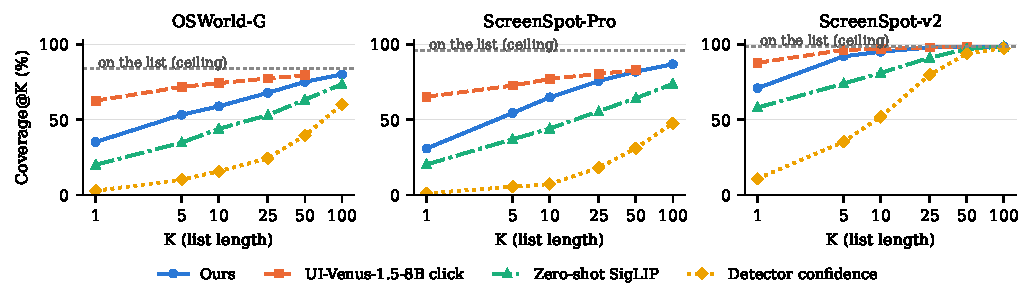
\includegraphics[width=\linewidth]{fig/cov_k.pdf}
\caption{\textbf{Coverage vs.\ list length} (leakage-filtered). Ours: 0.66 / 1.60 / 0.32~s per screen on an A10G; UI-Venus-1.5-8B's click turned into a ranking by distance: 1.57 / 2.98 / 2.16~s. The grounder is ahead at small $K$; at $K{=}50$ the gap is 4.3 / 1.0 / $-$0.3 points, at 1.9--6.8$\times$ lower cost, and fusing both is best (\cref{tab:grounders}). Dashed: the target is on the candidate list at all.}
\label{fig:covk}
\end{figure*}


\paragraph{What is still missed.}
On \sspro, almost all listed targets that our ranker places beyond 50 are small icons (target area below
$10^{-4}$ of the screen) on screens with more than 400 candidates. Recognising them requires knowing an
application's icon vocabulary, such as ``generate bitstream'' in Vivado or ``mark dimensions'' in SolidWorks, where
\cov{50} is only 42\%. On \osw, most remaining misses are relational instructions (``the second column of the
31st row'', ``the other text box'', ``the next slide''), which a ranker that scores each candidate independently
cannot resolve. A further 16\% of \osw targets are never listed: positions inside a slider or scrollbar, resize
grips and character spans. The supplement breaks coverage down by application group, element type and target size
(\cref{sec:supp-category}).

\subsection{Comparison with GUI grounding models}
\label{sec:grounders}

\begin{table*}[t]
\centering
\small
\setlength{\tabcolsep}{3.5pt}
\begin{tabular}{l c ccc ccc ccc}
\toprule
& & \multicolumn{3}{c}{\osw} & \multicolumn{3}{c}{\sspro} & \multicolumn{3}{c}{\ssv} \\
\cmidrule(lr){3-5}\cmidrule(lr){6-8}\cmidrule(lr){9-11}
Method & Params & click@1 & \cov{10} & \cov{50} & click@1 & \cov{10} & \cov{50} & click@1 & \cov{10} & \cov{50} \\
\midrule
TinyClick~\cite{pawlowski2024tinyclick} & 0.27B & 23.5 & 37.4 & 56.1 & 3.8 & 9.4 & 29.2 & 81.6 & 86.5 & 95.7 \\
ShowUI-2B~\cite{lin2025showui} & 2B & 21.0 & 48.6 & 66.3 & 7.6 & 40.8 & 59.4 & 76.7 & 91.1 & 96.9 \\
Qwen3-VL-2B & 2B & 32.4 & 45.3 & 60.9 & 30.2 & 45.6 & 61.8 & 81.6 & 88.3 & 96.6 \\
GUI-Actor-2B~\cite{wu2025guiactor} & 2B & 39.5 & 54.5 & 67.2 & 35.6 & 51.2 & 63.6 & 89.3 & 93.9 & 97.2 \\
UI-Venus-1.5-2B~\cite{gu2025uivenus} & 2B & 64.4 & 67.2 & 75.1 & 59.2 & 68.8 & 78.8 & 95.4 & 95.7 & 97.2 \\
UI-Venus-1.5-8B~\cite{gu2025uivenus} & 8B & 74.2 & 74.2 & 79.4 & 69.8 & 77.0 & 82.8 & 96.9 & 96.9 & 98.2 \\
\midrule
\textbf{Ours} & 0.2B & -- & 58.8 & 75.1 & -- & 64.8 & 81.8 & -- & 95.1 & 98.5 \\
Ours + UI-Venus-1.5-2B (fused) & & -- & 71.1 & 79.2 & -- & 72.8 & 88.4 & -- & 96.9 & 98.5 \\
Ours + UI-Venus-1.5-8B (fused) & & -- & \textbf{75.7} & \textbf{81.5} & -- & \textbf{77.8} & \textbf{89.0} & -- & \textbf{97.2} & \textbf{98.5} \\
\bottomrule
\end{tabular}
\caption{\textbf{Grounders as list builders.} click@1: the grounder's own click lands in the answer box.
\cov{K}: its click turned into a ranking of our candidates (candidates containing the click first, then by
distance). Fused: our score plus a Gaussian bonus around the click (fixed weight 5, width 0.5\% of the screen
diagonal for all benchmarks). All models run on the same instructions on one A10G; median latencies per
instruction in \cref{tab:speed}.}
\label{tab:grounders}
\end{table*}

Grounding models are trained to output one point, and every point induces a ranking: candidates under the point
first, then the rest by distance. \Cref{tab:grounders} evaluates six open grounders this way under our protocol.
Small, fast grounders (TinyClick, ShowUI) produce poor lists on dense screens because their single point says
little about the rest of the screen; their \cov{50} on \sspro is 29--59\%. Our ranker produces better lists than
every grounder up to 2B parameters except UI-Venus-1.5, at 2.3--9$\times$ lower latency than GUI-Actor-2B and
Qwen3-VL-2B (\cref{tab:speed}).

UI-Venus-1.5 is a much stronger grounder. Its click lands on the target for 74.2\% of \osw instructions, more than
our \cov{25}, but it fails on different instructions than our ranker. Adding a bonus around the grounder's click to
our scores gives the best lists at every $K$ on all three benchmarks: with UI-Venus-1.5-8B, \cov{10} rises to 75.7
/ 77.8 / 97.2\% and \cov{50} to 81.5 / 89.0 / 98.5\%. A list-based agent gets the grounder's pick first when it is
right. When it is wrong (26\% of \osw and 30\% of \sspro instructions), our ranking still has the target in its
top 10 for 25\% / 40\% of these misses and in its top 50 for 53\% / 64\%, which gives a selector a second chance.
Many of the remaining misses have no matching candidate at all (34\% of the UI-Venus-1.5-8B misses on \osw), and
no reordering can fix those.

\subsection{Downstream: a fixed selector}
\label{sec:selector}

Coverage is a proxy for whether the model that chooses from the list chooses correctly. To measure that directly,
we keep the selector fixed (Qwen2.5-VL-7B-Instruct without any fine-tuning) and vary only the list it receives. The selector
sees the screenshot (at most $1280\cdot28^2$ pixels), the instruction and the numbered options, each with its label
(OCR text, or the Florence-2 caption for icons) and its box, and answers with a number.

\begin{table*}[t]
\centering
\small
\setlength{\tabcolsep}{4pt}
\begin{tabular}{l rrrr rrrr rrrr}
\toprule
& \multicolumn{4}{c}{\osw} & \multicolumn{4}{c}{\sspro} & \multicolumn{4}{c}{\ssv} \\
\cmidrule(lr){2-5}\cmidrule(lr){6-9}\cmidrule(lr){10-13}
List given to the selector & cov. & acc. & ms & tok. & cov. & acc. & ms & tok. & cov. & acc. & ms & tok. \\
\midrule
Full list, unranked & 83.8 & 24.3 & 2118 & 6698 & 96.0 & 9.4 & 4043 & 13316 & 98.5 & 79.4 & 1004 & 2573 \\
Confidence, top 10 & 15.6 & 12.5 & 760 & 1562 & 7.2 & 4.2 & 763 & 1597 & 51.8 & 45.7 & 761 & 1609 \\
Confidence, top 50 & 39.5 & 20.8 & 1040 & 2607 & 31.0 & 12.8 & 1048 & 2685 & 93.9 & 76.7 & 995 & 2564 \\
Ours, top 5 & 53.2 & 37.8 & 729 & 1445 & 54.4 & 33.4 & 738 & 1457 & 92.0 & 79.4 & 742 & 1484 \\
Ours, top 10 & 58.8 & 37.6 & 760 & 1578 & 64.8 & \textbf{34.6} & 762 & 1595 & 95.1 & 80.1 & 761 & 1615 \\
Ours, top 25 & 67.8 & \textbf{38.5} & 841 & 1992 & 75.6 & 34.2 & 851 & 2008 & 97.9 & \textbf{81.0} & 843 & 2027 \\
Ours, top 50 & 75.1 & 37.4 & 1030 & 2690 & 81.8 & 31.6 & 1036 & 2702 & 98.5 & 79.4 & 1004 & 2564 \\
\bottomrule
\end{tabular}
\caption{\textbf{A fixed selector choosing from different lists} (Qwen2.5-VL-7B-Instruct, not fine-tuned;
leakage-filtered instructions as in \cref{tab:main}). cov.: a target is on the list; acc.: the selector picks a
target; ms: selector latency, median; tok.: prompt length, median. On \sspro, 4 of the 500 full lists do not fit
in GPU memory even with labels shortened to 25 characters; they count as errors.}
\label{tab:selector}
\end{table*}

The same selector does better with a better list (\cref{tab:selector}). On \osw, given every candidate, the
selector finds the target only 24.3\% of the time, although the target is on the list 83.8\% of the time: with 190
options it is right in only 29\% of the cases where it could be. Our top-10 list contains the target less often
(58.8\%), but the selector picks it far more reliably, for 37.6\% accuracy, with 4.2$\times$ fewer prompt tokens
and a 2.8$\times$ faster selector. The effect is larger on \sspro, where screens carry 442 candidates. There the
full list (13k tokens) gives 9.4\% and our top 10 gives 34.6\%, a 3.7$\times$ improvement with 8$\times$ fewer
tokens and a 5.3$\times$ faster selector. Shortening the list alone does not help: the top 10 by detector
confidence gives 12.5\% and 4.2\%. Accuracy is nearly flat from $K{=}5$ to $K{=}50$, because the gain in coverage is
offset by a harder choice (on \osw, accuracy when the target is listed falls from 71\% at $K{=}5$ to 50\% at
$K{=}50$). In practice $K$ can therefore be set by the latency and captioning budget. On \ssv, with 47 candidates
per screen, the full list is already short, and our top 10 matches its accuracy (80.1\% vs.\ 79.4\%) with
1.6$\times$ fewer tokens. Ranking helps most on dense screens.

A 7B selector choosing from our list remains below the best single-point grounders on these benchmarks
(UI-Venus-1.5-2B clicks correctly 64.4\% of the time on \osw). This experiment isolates the effect of the list. It
does not show that an untrained selector choosing from a list beats a trained grounder. Two ways to combine both
are selectors trained for option lists and the fused lists of \cref{sec:grounders}, which put a grounder's click
first and our ranked alternatives after it.

\subsection{Latency}
\label{sec:speed}

\begin{table}[t]
\centering
\small
\setlength{\tabcolsep}{4pt}
\begin{tabular}{l rrr}
\toprule
Stage (median ms) & OSW-G & SS-Pro & SS-v2 \\
\midrule
Candidates per screen & 190 & 442 & 47 \\
OCR (laptop)$^\dagger$ & 150 & 213 & 140 \\
Detection (2 detectors) & 190 & 254 & 179 \\
Merge & 14 & 35 & 4 \\
Context crops (GPU) & 15 & 43 & 8 \\
Image embeddings & 485 & 1121 & 120 \\
Text embedding + ranking & 11 & 12 & 11 \\
\textbf{Total (GPU)} & \textbf{656} & \textbf{1596} & \textbf{318} \\
\midrule
TinyClick & 132 & 151 & 140 \\
ShowUI-2B & 749 & 768 & 752 \\
UI-Venus-1.5-2B & 874 & 2614 & 1182 \\
GUI-Actor-2B & 1729 & 8694 & 2872 \\
Qwen3-VL-2B & 2433 & 3743 & 2414 \\
UI-Venus-1.5-8B & 1569 & 2976 & 2160 \\
\bottomrule
\end{tabular}
\caption{\textbf{Latency} per instruction on one A10G (OSW-G: \osw, SS-Pro: \sspro, SS-v2: \ssv; 100 screens per benchmark for ours, the 500 evaluation
instructions for the grounders, batch size 1). $^\dagger$OCR runs on the device that captured the screen,
concurrently with detection, and is not part of the GPU total.}
\label{tab:speed}
\end{table}

\Cref{tab:speed} breaks down our latency. Embedding the candidate crops takes most of the time and grows with the
number of candidates: 485~ms for the 190 candidates of a median \osw screen and 1.1~s for the 442 of a \sspro
screen. Two implementation choices matter. Cutting, resizing and normalising all crops on the GPU in one batched
\texttt{roi\_align} instead of with PIL removes about 0.5~s of CPU preprocessing per \sspro screen and changes
\cov{50} by at most 0.8 points (\cref{tab:ablations}). A vectorised merge gives identical lists in a tenth of the
time. End to end, our list costs 0.3--1.6~s per screen, 1.3--3.7$\times$ less than UI-Venus-1.5-2B and
1.9--6.8$\times$ less than UI-Venus-1.5-8B on the same GPU. The image embeddings can be reused, so a further
instruction on the same screen costs 11~ms. Labelling adds about 2~ms per captioned icon: on a median \sspro screen,
captioning the 43 icons in our top 50 takes about 90~ms, against about 0.7~s for all 347 icons (measured on 28
\sspro screens).

\subsection{Ablations}
\label{sec:ablations}

\begin{table}[t]
\centering
\small
\setlength{\tabcolsep}{2.5pt}
\begin{tabular}{l cc cc cc}
\toprule
& \multicolumn{2}{c}{OSW-G} & \multicolumn{2}{c}{SS-Pro} & \multicolumn{2}{c}{SS-v2} \\
\cmidrule(lr){2-3}\cmidrule(lr){4-5}\cmidrule(lr){6-7}
Variant & @10 & @50 & @10 & @50 & @10 & @50 \\
\midrule
Ours (384 px, 3 epochs) & 58.8 & 75.1 & 64.8 & 81.8 & 95.1 & 98.5 \\
\quad tight crops & 59.3 & 72.8 & 61.6 & 78.4 & 94.8 & 98.2 \\
\quad 224 px, 3 epochs & 61.1 & 74.4 & 58.2 & 77.4 & 94.8 & 98.2 \\
\quad 224 px, epoch 1 of 3 & 59.0 & 71.7 & 56.4 & 75.4 & 92.9 & 98.2 \\
\quad 224 px, 1 epoch & 60.9 & 73.2 & 60.0 & 76.6 & 94.2 & 98.2 \\
\qquad tight crops & 58.4 & 71.9 & 64.2 & 79.8 & 94.5 & 98.2 \\
\qquad sigmoid loss & 60.3 & 74.0 & 60.6 & 76.8 & 92.6 & 98.2 \\
\quad SigLIP2-so400m, 224$^\ast$ & 48.0 & 68.8 & 62.4 & 78.6 & 94.5 & 98.2 \\
\quad + Windows data$^\dagger$ & 62.2 & 74.8 & 65.6 & 82.2 & 95.1 & 98.5 \\
\quad GPU crops & 59.0 & 75.1 & 64.8 & 81.0 & 94.8 & 98.5 \\
\quad zero-shot, 384 & 43.9 & 63.2 & 44.0 & 64.2 & 81.0 & 96.9 \\
\bottomrule
\end{tabular}
\caption{\textbf{Ablations} (\cov{10} / \cov{50}, leakage-filtered). $^\ast$Lower 12 layers and embeddings frozen
to fit one 24\,GB GPU; saving the second epoch's checkpoint failed (disk full), so the evaluated weights are most likely the first epoch's. $^\dagger$7,651 training screens instead of 4,816, adding 2,979 OS-Atlas Windows screens; not used in the frozen model reported elsewhere.}
\label{tab:ablations}
\end{table}

\paragraph{Resolution.} Input resolution matters most on \sspro, where targets are smallest: going from 224 to
384 px adds 6.6 points of \cov{10} and 4.4 of \cov{50}, and changes \osw and \ssv by at most 2.3 points. Training
longer at 224 px helps on all three benchmarks (epoch 1 vs.\ epoch 3 of the same run).

\paragraph{Context vs.\ tight crops.} Without fine-tuning, the context window helps on \osw (+5.4 \cov{10},
\cref{tab:main}), where instructions often refer to an element's surroundings. After fine-tuning at 224 px the
results are mixed: context crops are better on \osw (+2.5 / +1.3) and worse on \sspro ($-$4.2 / $-$3.2). At 224 px
input, a window three times the element's size leaves a 16 px icon only a few pixels wide, so on \sspro the context
costs detail. At 384 px this cost disappears. Against tight crops trained identically, context crops gain 3.2 /
3.4 points on \sspro and 2.3 points of \cov{50} on \osw, and are within 0.5 points elsewhere. Context crops and the
higher resolution work together, which is why our model uses both.

\paragraph{Loss, data, encoder.} The per-screen listwise loss and a per-pair sigmoid loss perform alike (within
1.6 points everywhere). Both draw their negatives from the same screen, which seems to be the part that matters.
More data helps a little: adding 2,979 Windows screens raises \cov{10} by 3.4 points on \osw and 0.8 on \sspro,
with \cov{50} within 0.4 points. All other results use the model trained without them. A larger encoder does not
help within our budget: SigLIP2-so400m, with its lower half frozen to fit one 24\,GB GPU, is worse than the base
model on \osw and \sspro.

\paragraph{GPU crops.} Cutting and resizing crops on the GPU (\texttt{roi\_align}) instead of with PIL changes
\cov{50} by at most 0.8 points and removes the CPU preprocessing cost.

\section{Limitations and conclusion}
\label{sec:conclusion}

\paragraph{Limitations.}
Our ranker scores candidates independently, so instructions defined by layout (``the third row'') are hard for it;
a set-level second stage over the top candidates could address them. Targets that are not elements at all, such as
a position along a slider, never enter the list. Coverage is measured against benchmark answer boxes matched to
candidates, which can over- or under-count when boxes nest. We also evaluate single decisions, not multi-step task
success.

\paragraph{Conclusion.}
We built the screen's option list from pixels, ranked it for the instruction before labelling anything, and judged
it by whether the needed element is on a short list. A context-crop SigLIP ranker trained with a per-screen
listwise loss raises \cov{50} on \sspro from 31\% to 82\% and needs up to 8$\times$ fewer captions. Its rankings
complement single-point grounders: fused with a grounder's click, they give a selector alternatives to recover from
when the click is wrong. With the selector held fixed, the shorter ranked list is also more accurate: on \sspro an
off-the-shelf VLM goes from 9.4\% with every candidate to 34.6\% with our top 10.

{
    \small
    \bibliographystyle{ieeenat_fullname}
    \bibliography{main}
}
% Supplementary material (split off into its own PDF for submission)
\clearpage
\setcounter{page}{1}
\maketitlesupplementary

\section{Coverage by category}
\label{sec:supp-category}

\Cref{tab:supp-category} breaks down the coverage of our frozen ranker (\cref{tab:main}) by the categories the
benchmarks annotate, next to UI-Venus-1.5-8B's single click (\cref{tab:grounders}). For \osw, which has no comparable
category field, we bin targets by area as a share of the screen (442 of the 481 instructions have a box target;
the rest are polygons).

\begin{table}[h]
\centering
\small
\setlength{\tabcolsep}{3.5pt}
\begin{tabular}{l r rrr r}
\toprule
Subset & $n$ & listed & \cov{10} & \cov{50} & Venus@1 \\
\midrule
\multicolumn{6}{l}{\emph{\osw, by target area}} \\
\quad all & 481 & 83.8 & 58.8 & 75.1 & 74.2 \\
\quad $<0.01\%$ & 31 & 19.4 & 16.1 & 19.4 & 38.7 \\
\quad $0.01$--$0.1\%$ & 241 & 82.6 & 53.9 & 73.4 & 68.9 \\
\quad $\ge 0.1\%$ & 170 & 95.3 & 68.2 & 83.5 & 83.5 \\
\midrule
\multicolumn{6}{l}{\emph{\sspro}} \\
\quad all & 500 & 96.0 & 64.8 & 81.8 & 69.8 \\
\quad CAD & 82 & 93.9 & 41.5 & 67.1 & 64.6 \\
\quad Creative & 111 & 94.6 & 66.7 & 78.4 & 63.1 \\
\quad Dev & 95 & 95.8 & 62.1 & 83.2 & 68.4 \\
\quad Office & 69 & 97.1 & 76.8 & 94.2 & 89.9 \\
\quad OS & 58 & 98.3 & 75.9 & 89.7 & 74.1 \\
\quad Scientific & 85 & 97.6 & 70.6 & 83.5 & 65.9 \\
\quad text targets & 301 & 96.7 & 73.1 & 85.7 & 85.7 \\
\quad icon targets & 199 & 95.0 & 52.3 & 75.9 & 45.7 \\
\midrule
\multicolumn{6}{l}{\emph{\ssv}} \\
\quad all & 326 & 98.5 & 95.1 & 98.5 & 96.9 \\
\quad desktop & 130 & 99.2 & 96.2 & 99.2 & 98.5 \\
\quad mobile & 157 & 98.1 & 94.3 & 98.1 & 96.8 \\
\quad web & 39 & 97.4 & 94.9 & 97.4 & 92.3 \\
\quad text targets & 192 & 99.5 & 98.4 & 99.5 & 99.0 \\
\quad icon targets & 134 & 97.0 & 90.3 & 97.0 & 94.0 \\
\bottomrule
\end{tabular}
\caption{\textbf{Coverage by category} (leakage-filtered). listed: the target is among all candidates;
Venus@1: UI-Venus-1.5-8B's click lands on the target.}
\label{tab:supp-category}
\end{table}

\emph{Tiny targets are lost before ranking.} On \osw, targets below $0.01\%$ of the screen are listed only 19\% of
the time, and every listed one is in our top 50. These are slider positions, resize grips and character spans that
no detector boxes.

\emph{A ranked list helps most for icons.} On \sspro icon targets, our top 50 contains the target 75.9\% of the
time, while the grounder's single click is right 45.7\% of the time. On text targets the two are level (85.7\%).

\emph{CAD is the hardest domain.} Its targets are listed as often as elsewhere (93.9\%), but they are small,
unlabelled tool icons whose meaning depends on the application, and \cov{50} drops to 67\%.

\end{document}
